\documentclass[../../main/main.tex]{subfiles}
\graphicspath{{./figures/}}

\dominitoc
\faketableofcontents

\renewcommand{\mtcSfont}{\small\bfseries}
\renewcommand{\mtcSSfont}{\footnotesize}
\mtcsettitle{minitoc}{}
\mtcsetrules{*}{off}

\makeatletter
\renewcommand{\@chapapp}{Induction -- chapitre}
\makeatother

% \toggletrue{student}
% \toggletrue{corrige}
% \renewcommand{\mycol}{black}
% \renewcommand{\mycol}{gray}

\hfuzz=5.003pt

\begin{document}
\setcounter{chapter}{3}

\settype{book}
\settype{prof}
\settype{stud}

\chapter{Conversion de puissance électromécanique}
\label{ch:convelecmeca}
% \epigraph{\openquote\textit{%
% 		Sire, je n'avais pas besoin de cette hypothèse.
% 	}%
% 	\closequote}{Pierre-Simon \textsc{Laplace} à \textsc{Napoléon}, \textit{circa} 1800}

\vspace*{\fill}

\begin{tcn}(appl)<ctc>"somm"'t'{Sommaire}
	\let\item\olditem
	\vspace{-15pt}
	\minitoc
	\vspace{-25pt}
\end{tcn}

\begin{tcn}[fontupper=\small](appl)<ctc>"how"'t'{Capacités exigibles}
	\tcbsubtitle{\fatbox{Rails de \textsc{Laplace} et spire rectangulaire en rotation}}
	\begin{itemize}[label=\rcheck]
		\item Interpréter qualitativement les phénomènes observés.
		\item Écrire les équations électrique et mécanique en précisant les
		      conventions de signe.
		\item Effectuer un bilan énergétique.
		\item Citer des applications dans le domaine de l'industrie ou de la vie
		      courante.
		\item Expliquer l'origine des courants de \textsc{Foucault} et en citer des
		      exemples d'utilisation.
	\end{itemize}
\end{tcn}

\vspace{-15pt}

% \vspace*{\fill}
%
% \newpage
%
% \vspace*{\fill}
% {%
% \begin{boxes}
\begin{tcn}[sidebyside, fontupper=\small, fontlower=\small](appl)<ctb>"chek"'t'{L'essentiel}
	\begin{tcn}(defi)<ctc>'t'{Définitions}
		\tcblistof[\paragraph*]{defi}{\hspace*{4.8pt}}
	\end{tcn}
	% \begin{tcn}(rapp)<ctc>'t'{Rappels}
	% 	\tcblistof[\paragraph*]{rapp}{\hspace*{4.8pt}}
	% \end{tcn}
	\begin{tcn}(prop)<ctc>'t'{Propriétés}
		\tcblistof[\paragraph*]{prop}{\hspace*{4.8pt}}
		\tcblistof[\paragraph*]{loi}{\hspace*{4.8pt}}
		% \tcblistof[\paragraph*]{theo}{\hspace*{4.8pt}}
	\end{tcn}
	% \begin{tcn}(coro)<ctc>'t'{Corollaires}
	%   \tcblistof[\paragraph*]{coro}{\hspace*{4.8pt}}
	% \end{tcn}
	% \begin{tcn}(demo)<ctc>'t'{Démonstrations}
	% 	\tcblistof[\paragraph*]{demo}{\hspace*{4.8pt}}
	% 	\tcblistof[\paragraph*]{prev}{\hspace*{4.8pt}}
	% \end{tcn}
	% \begin{tcn}(inte)<ctc>'t'{Interprétations}
	% 	\tcblistof[\paragraph*]{inte}{\hspace*{4.8pt}}
	% \end{tcn}
	\begin{tcn}(impl)<ctc>'t'{Implications}
		\tcblistof[\paragraph*]{impl}{\hspace*{4.8pt}}
	\end{tcn}
	% \begin{tcn}(tool)<ctc>'t'{Outils}
	% 	\tcblistof[\paragraph*]{tool}{\hspace*{4.8pt}}
	% \end{tcn}
	% \begin{tcn}(nota)<ctc>'t'{Notations}
	%   \tcblistof[\paragraph*]{nota}{\hspace*{4.8pt}}
	% \end{tcn}
	% \begin{tcn}(appl)<ctc>'t'{Applications}
	% 	\tcblistof[\paragraph*]{appl}{\hspace*{4.8pt}}
	% \end{tcn}
	% \begin{tcn}(rema)<ctc>'t'{Remarques}
	%   \tcblistof[\paragraph*]{rema}{\hspace*{4.8pt}}
	% \end{tcn}
	% \begin{tcn}(exem)<ctc>'t'{Exemples}
	% 	\tcblistof[\paragraph*]{exem}{\hspace*{4.8pt}}
	% \end{tcn}
	% \begin{tcn}*(ror)<ctc>"hart"'t'{Points importants}
	%   \tcblistof[\paragraph*]{ror}{\hspace*{4.8pt}}
	% \end{tcn}
	% \begin{tcn}(impo)<ctc>'t'{Erreurs communes}
	%   \tcblistof[\paragraph*]{impo}{\hspace*{4.8pt}}
	% \end{tcn}
	\tcblower
	% \begin{tcn}(defi)<ctc>'t'{Définitions}
	%   \tcblistof[\paragraph*]{defi}{\hspace*{4.8pt}}
	% \end{tcn}
	% \begin{tcn}(rapp)<ctc>'t'{Rappels}
	%   \tcblistof[\paragraph*]{rapp}{\hspace*{4.8pt}}
	% \end{tcn}
	% \begin{tcn}(prop)<ctc>'t'{Propriétés}
	%   \tcblistof[\paragraph*]{prop}{\hspace*{4.8pt}}
	%   \tcblistof[\paragraph*]{loi}{\hspace*{4.8pt}}
	%   \tcblistof[\paragraph*]{theo}{\hspace*{4.8pt}}
	% \end{tcn}
	% \begin{tcn}(coro)<ctc>'t'{Corollaires}
	%   \tcblistof[\paragraph*]{coro}{\hspace*{4.8pt}}
	% \end{tcn}
	% \begin{tcn}(demo)<ctc>'t'{Démonstrations}
	% 	\tcblistof[\paragraph*]{demo}{\hspace*{4.8pt}}
	% 	\tcblistof[\paragraph*]{prev}{\hspace*{4.8pt}}
	% \end{tcn}
	% \begin{tcn}(inte)<ctc>'t'{Interprétations}
	% 	\tcblistof[\paragraph*]{inte}{\hspace*{4.8pt}}
	% \end{tcn}
	% \begin{tcn}(impl)<ctc>'t'{Implications}
	% 	\tcblistof[\paragraph*]{impl}{\hspace*{4.8pt}}
	% \end{tcn}
	% \begin{tcn}(tool)<ctc>'t'{Outils}
	%   \tcblistof[\paragraph*]{tool}{\hspace*{4.8pt}}
	% \end{tcn}
	% \begin{tcn}(nota)<ctc>'t'{Notations}
	%   \tcblistof[\paragraph*]{nota}{\hspace*{4.8pt}}
	% \end{tcn}
	% \begin{tcn}(odgr)<ctc>'t'{Ordres de grandeur}
	% 	\tcblistof[\paragraph*]{odgr}{\hspace*{4.8pt}}
	% \end{tcn}
	% \begin{tcn}(appl)<ctc>'t'{Applications}
	% 	\tcblistof[\paragraph*]{appl}{\hspace*{4.8pt}}
	% \end{tcn}
	% \begin{tcn}(rema)<ctc>'t'{Remarques}
	%   \tcblistof[\paragraph*]{rema}{\hspace*{4.8pt}}
	% \end{tcn}
	% \begin{tcn}(exem)<ctc>'t'{Exemples}
	% 	\tcblistof[\paragraph*]{exem}{\hspace*{4.8pt}}
	% \end{tcn}
	\begin{tcn}*(ror)<ctc>"hart"'t'{Points importants}
		\tcblistof[\paragraph*]{ror}{\hspace*{4.8pt}}
	\end{tcn}
	\begin{tcn}(impo)<ctc>'t'{Erreurs communes}
		\tcblistof[\paragraph*]{impo}{\hspace*{4.8pt}}
	\end{tcn}
\end{tcn}
% \end{boxes}
% }%

\vspace*{\fill}
\newpage

\section{Principe de la conversion de puissance}
% \section{Conversion de puissance électrique en puissance mécanique}
\label{sec:convelecmeca}
\subsection{Vocabulaire}
\label{ssec:voca}

On a vu précédemment quelques exemples où un mouvement mécanique créé un champ
électrique, mais également l'inverse. Un peu de vocabulaire~:
\begin{itemize}
	\item On parle de circuit \textbf{moteur} lorsqu'il convertit une puissance
	      de \textbf{électrique à mécanique}~;
	\item On parle de circuit \textbf{générateur} lorsqu'il convertit une puissance
	      de \textbf{mécanique à électrique}.
\end{itemize}
\begin{figure}[h]
	\centering
	\noindent
	\begin{minipage}[c]{.48\linewidth}
		\sswitch{
			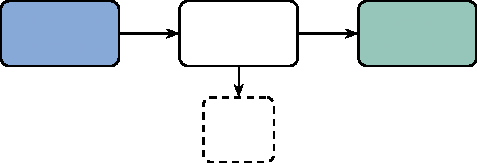
\includegraphics[width=\linewidth]{motdef_stud}
		}{
			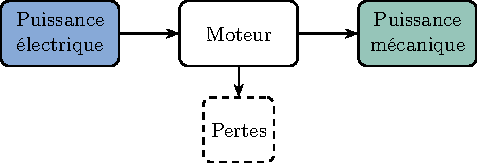
\includegraphics[width=\linewidth]{motdef_prof}
		}%
	\end{minipage}
	\hfill
	\begin{minipage}[c]{.48\linewidth}
		\sswitch{
			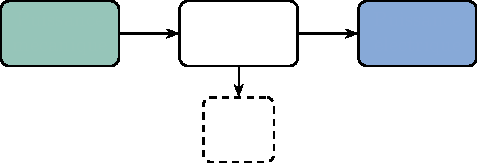
\includegraphics[width=\linewidth]{genedef_stud}
		}{
			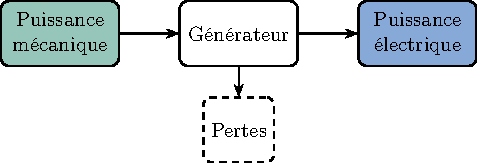
\includegraphics[width=\linewidth]{genedef_prof}
		}%
	\end{minipage}
	\caption{Schématisation des fonctionnements moteur et générateur.}
	\label{fig:motgene}
\end{figure}
\vspace*{-20pt}

\subsection{Exemple des rails de \textsc{Laplace} moteurs}
\label{ssec:rlplmot}
\begin{tcb*}(defi){Rails de \textsc{Laplace} moteurs}
	Les rails de \textsc{Laplace} \textbf{moteurs} sont deux conducteurs
	rectilignes parallèles reliés par une tige mobile conductrice rendant le
	circuit \textbf{déformable}, plongé dans un champ magnétique constant
	perpendiculaire au circuit et \textbf{alimenté par une f.é.m.\ constante
		$U_0$}.
\end{tcb*}
\noindent
\begin{minipage}[c]{.50\linewidth}
	Le générateur étant dans un circuit fermé, il impose un courant $i > 0$.
	\textbf{On néglige l'auto-induction}, et on appelle $R$ la résistance totale du
	circuit. Nous avons déjà constaté expérimentalement la mise en mouvement de la
	barre à l'aide de la force de \textsc{Laplace}. Quelle vitesse atteint-elle~?
\end{minipage}
\hfill
\begin{minipage}[c]{.50\linewidth}
	\begin{center}
		\sswitch{
			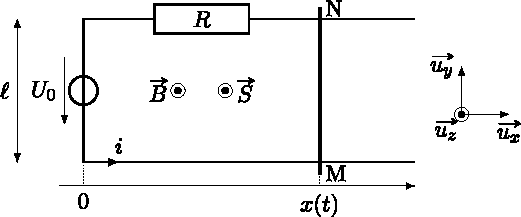
\includegraphics[scale=1, draft=true]{rlplmot_schema}
		}{
			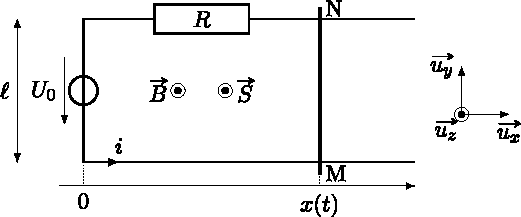
\includegraphics[scale=1]{rlplmot_schema}
		}%
		\captionof{figure}{Rails de \textsc{Laplace} moteurs.}
		\label{fig:rlplmot_schema}
	\end{center}
\end{minipage}
% \vspace*{-20pt}

\subsubsection{Analyse qualitative}
\label{ssec:rlplmot_anaqual}
\begin{figure}[H]
	\centering
	\sswitch{
		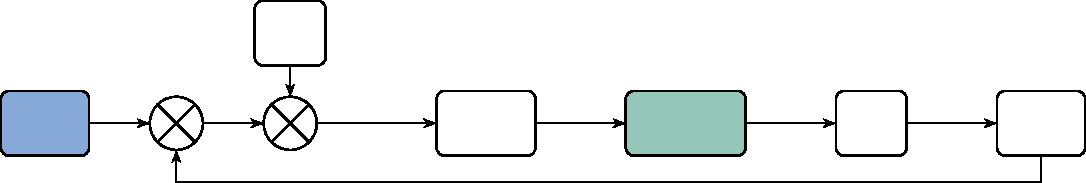
\includegraphics[scale=1]{modlenz-rlplmot_stud}
	}{
		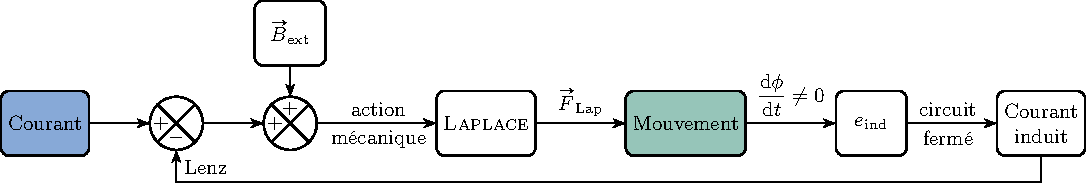
\includegraphics[scale=1]{modlenz-rlplmot_prof}
	}%
	\caption{Schéma de causalité des conséquences de l'induction.}
	\label{fig:modlenz_rlplmot}
\end{figure}
Avant de se lancer dans les calculs, on peut déterminer le comportement du
système avec la loi de \textsc{Lenz}.
\begin{enumerate}
	\item À l'origine de l'induction est la présence d'un champ extérieur
	      $\vv{B\ind{ext}}$ et d'un courant dans le circuit.

	\item Combinés ensemble, ils appliquent une action de \textsc{Laplace} sur le
	      barreau, le mettant en mouvement et \textbf{déformant} le circuit.

	\item Il y a donc \textbf{variation du flux}, et d'après la loi de
	      \textsc{Faraday} une f.é.m.\ induite y apparaît.

	\item Le circuit étant toujours fermé, il y a également un courant induit.
\end{enumerate}
L'induction modérant, par ses conséquences, les causes qui lui ont donné
naissance, on en conclut que ce \textbf{courant induit s'oppose au courant
	initial}, ce qui générera une force de \textsc{Laplace} opposée tendant à
freiner l'accélération du barreau.
On veut étudier ce comportement et notamment
connaître la vitesse finale~: est-elle infinie~? nulle~? constante~?

\begin{tcb*}[cnt](impo){Comparaisons en induction}
	\psw{%
		Une étude de causalité doit comparer une conséquence et une cause de
		mêmes natures~!
	}%
\end{tcb*}

\subsubsection{Analyse mécanique}
\label{sssec:rlplmot_anameca}
On étudie le mouvement de la barre de masse $m$ dans le référentiel de la
salle de classe. Avec un bilan des forces~:
\begin{itemize}
	\item[b]{\psw{Poids}} \psw{%
		$\vv{P} = m \vv{g} = -mg\uz$~;
	}%
	\item[b]{\psw{Réaction normale}} \psw{%
		$\vv{N} = N\uz$~;
	}%
	\item[b]{\psw{Force de \textsc{Laplace}}} \psw{%
		$\vv{F\ind{Lap}} = i \vv{\rm MN}\wedge \vv{B} = i \ell B \ux$~;
	}%
	\item[b]{\psw{Frottements}} \psw{%
		$\vv{F_f} = -F_f \ux$ avec $F_f > 0$.
	}%
\end{itemize}
Ainsi,
\psw{%
	\[
		m \dv{\vv{v}}{t} = \vv{P} + \vv{F\ind{Lap}} + \vv{N} + \vv{F_f}
	\]
}%
D'où, en projetant sur $\ux$~:
\begin{tcb}(prop){Équation mécanique}
	\psw{%
		\begin{equation}
			\usetagform{black}
			\label{eq:eqmeca}
			m \dv{v}{t} = i \ell B - F_f
		\end{equation}
		\vspace*{-10pt}
	}%
\end{tcb}

\subsubsection{Analyse électrique}
\label{sssec:rlplmot_anaelec}
La déformation du circuit entraîne une variation de sa surface. Ainsi, même avec
un champ magnétique constant, le flux magnétique varie, impliquant l'apparition
d'une f.é.m.\ induite.
\bigbreak
\noindent
Avec $\vv{S} = S\uz$ pris dans le sens de $i$, on trouve pour $\F$~:
\psw{%
	\[
		\F = B\uz \cdot S\uz = BS = B \ell x
	\]
}%
D'où, avec la loi de \textsc{Faraday}~:
\psw{%
	\[
		e = -\dv{\F}{t} = -B \ell \dot{x}
	\]
}%
Placée en \textbf{convention générateur}. Donc, avec la loi des mailles~:
\psw{%
	\[
		e+U_0 = Ri \quad \Ra \quad U_0 = Ri + B \ell \dot{x}
	\]
}%
Ainsi,
\begin{tcb}(prop){Équation électrique}
	\psw{%
		\begin{equation}
			\usetagform{black}
			\label{eq:eqelec}
			U_0 = Ri + B \ell v
		\end{equation}
		\vspace*{-10pt}
	}%
\end{tcb}

\subsubsection{Résolution}
\label{sssec:rlplmot_resol}
On cherche à éliminer $i$ pour obtenir une équation différentielle sur $v$. On
l'isole dans \eqref{eq:eqelec}~:
\psw{%
	\[
		i = \frac{U_0}{R} - \frac{B \ell }{R}v
	\]
}%
Et on substitue $i$ dans l'équation mécanique \eqref{eq:eqmeca} \textbf{en
	l'absence de frottements}~:
\psw{%
	\begin{align*}
		m \dv{v}{t}                                   & = \left( \frac{U_0}{R} - \frac{B \ell }{R} v \right) \ell B
		\\\Lra
		m \dv{v}{t}                                   & = \frac{U_0 \ell B}{R} - \frac{B^2 \ell ^{2}}{R}v
		\\\Lra
		\Aboxed{\dv{v}{t} + \frac{B^2 \ell ^{2}}{Rm}v & = \frac{U_0 \ell B}{Rm}}
	\end{align*}
}%
On obtient donc une équation différentielle de la forme~:
\psw{%
	\[
		\boxed{\dv{v}{t} + \frac{v}{\tau} = \frac{v\ind{lim}}{\tau}}
		\qav
		\boxed{\tau = \frac{Rm}{B^2 \ell ^{2}}}
		\qet
		\boxed{v\ind{lim} = \frac{U_0}{B \ell }}
	\]
}%
Qui se résout en
\psw{%
	\[
		\boxed{v(t) = v\ind{lim}\left( 1 - \exr^{-t/\tau} \right)}
		\Lra
		\boxed{i(t) = \frac{U_0}{R}\exr^{-t/\tau}}
	\]
}%
\begin{tcb*}(impl){Rails de \textsc{Laplace} moteurs}
	Ainsi, \psw{l'\textbf{intensité finit par être nulle} et \textbf{la vitesse du
			rail finit par atteindre une valeur limite}.}
\end{tcb*}

\subsubsection{Résumé méthode}
\label{sssec:rlplmot_mth}
\begin{tcb*}(ror){Méthode de résolution}
	\begin{enumerate}
		\item \psw{%
			      Obtenir l'équation mécanique~:
		      }%
		      \begin{itemize}
			      \item \psw{%
				            PFD si translation
			            }%
			      \item \psw{%
				            TMC si rotation
			            }%
		      \end{itemize}
		\item \psw{%
			      Obtenir l'équation électrique~:
		      }%
		      \begin{enumerate}
			      \item \psw{%
				            Définir un sens pour le courant, avoir $\vv{S}$, calculer $\F$~;
			            }%
			      \item \psw{%
				            Utiliser la loi de \textsc{Faraday} pour avoir la f.é.m.\ induite~;
			            }%
			      \item \psw{%
				            L'ajouter dans le circuit en \textbf{convention générateur}~;
			            }%
			      \item \psw{%
				            Appliquer la loi des mailles
			            }%
		      \end{enumerate}
		\item \psw{%
			      Résoudre les équations couplées
		      }%
	\end{enumerate}
\end{tcb*}

\subsubsection{Bilan énergétique}
\label{sssec:rlplmot_bilanrj}
\begin{itemize}
	\item[b]{Bilan électrique}: \psw{%
		On multiplie la LdM par $i$~:
		\[
			U_0i = Ri^2 + B \ell vi
		\]
	} On identifie~:
	\begin{itemize}
		\item puissance du générateur~: \psw{%
			      $\Pc\ind{gene}\sup{f} = U_0i$
		      }%
		\item puissance dissipée par effet \textsc{Joule}~: \psw{%
			      $\Pc_J\sup{r} = Ri^2$
		      }%
		\item puissance reçue par la f.é.m.~: \psw{%
			      $\Pc\ind{fem}\sup{r} = -ei = B \ell vi$
		      }%
	\end{itemize}
	Ainsi,
	\psw{%
		\[
			\boxed{\Pc\ind{gene}\sup{f} = \Pc_J\sup{r} + \Pc\ind{fem}\sup{r}}
		\]
	}%
	\item[b]{Bilan mécanique}: \psw{%
		On multiplie le PFD par $v$~:
		\[
			mv \dv{v}{t} = i \ell Bv - F_f v
			\Lra
			i \ell Bv = mv \dv{v}{t} + F_f v
		\]
	}%
	On identifie~:
	\begin{itemize}
		\item dérivée de l'énergie cinétique~: \psw{%
			      $\dv{\Ec_c}{t} = mv \dv{v}{t}$
		      }%
		\item puissance reçue des forces de \textsc{Laplace}~: \psw{%
			      $\Pc\ind{Lap}\sup{r} = i \ell Bv$
		      }%
		\item puissance dissipée par frottements~: \psw{%
			      $\Pc_f\sup{f} = -(-F_fv) = F_fv$
		      }%
	\end{itemize}
	Ainsi,
	\psw{%
		\[
			\boxed{\dv{\Ec_c}{t} + \Pc_f\sup{f} = \Pc\ind{Lap}\sup{r}}
		\]
	}%
\end{itemize}

\begin{tcb*}[sidebyside](ror){Bilan de puissance électromécanique}
	On remarque notamment que
	\psw{%
		\[
			\boxed{\Pc\ind{fem}\sup{reçue} = \Pc\ind{Lap}\sup{reçue}}
		\]
	}%
	C'est-à-dire que le \textbf{couplage électromécanique est parfait}~: la
	puissance électrique reçue par la force électromotrice induite est égale à la
	puissance mécanique (motrice) des forces de \textsc{Laplace}.
	\tcblower
	Cela s'étend à d'autres types de systèmes électromécaniques~:
	\psw{%
		\begin{gather*}
			\left\{
			\begin{array}{rcl}
				\Pc\ind{Lap}\sup{r} & = & \vv{F_L}\cdot \vf + \vv{\Gamma_L} \wedge \wf
				\\
				\Pc\ind{fem}\sup{f} & = & ei
			\end{array}
			\right.
			\\\Ra
			\boxed{\Pc\ind{Lap}\sup{r} + \Pc\ind{fem}\sup{f} = 0}
		\end{gather*}
	}%
\end{tcb*}

Ainsi, en définissant le rendement par
\[
	\boxed{\eta = \abs{\frac{\text{puissance utile}}{\text{puissance fournie}}}}
\]
on voit que \textbf{contrairement à la thermodynamique}, le \textbf{rendement
	théorique} de conversion électromécanique est de 1~! En effet, seules les
\textbf{pertes limitent le transfert}.

\subsubsection{Bilan global}
\label{sssec:rlplmot_bilanglb}
En combinant les résultats de puissance, on a mathématiquement puis
schématiquement~:
\psw{%
	\[
		\boxed{
			\Pc\ind{gene}\sup{f} =
			\underbracket[1pt]{\Pc\ind{utile}}_{\dv{\Ec_c}{t}} + \Pc_J\sup{r} +
			\Pc_f\sup{f}
		}
	\]
}%
\begin{figure}[H]
	\centering
	\sswitch{
		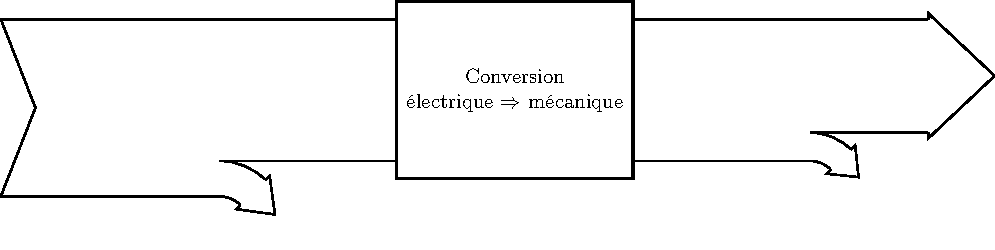
\includegraphics[width=\linewidth]{sankey_E-M_stud}
	}{
		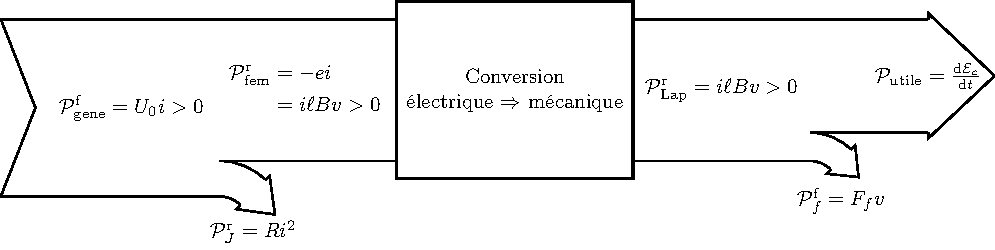
\includegraphics[width=\linewidth]{sankey_E-M_prof}
	}
	\vspace{-15pt}
	\captionof{figure}{Diagramme \textsc{Sankey} énergétique des rails de
		\textsc{Laplace} moteurs.}
	\label{fig:rlplmot_bilan}
\end{figure}

\subsection{Exemple des rails de \textsc{Laplace} générateurs}
\label{ssec:rlplgene}
\begin{tcb*}(defi){Rails de \textsc{Laplace} générateurs}
	Les rails de \textsc{Laplace} \textbf{générateurs} sont deux conducteurs
	rectilignes parallèles reliés par une tige mobile conductrice rendant le
	circuit \textbf{déformable}, plongé dans un champ magnétique constant
	perpendiculaire au circuit avec \textbf{une force $\vv{F} = F\,\ux$
		constante sur la tige}.
\end{tcb*}
\noindent
\begin{minipage}[c]{.50\linewidth}
	\textbf{On néglige l'auto-induction}, et on appelle $R$ la résistance totale du
	circuit. Nous pouvons constater expérimentalement que le déplacement du barreau
	est à l'origine d'un courant de quelques \si{\micro A} dans le circuit. On
	étudie alors le circuit ci-dessous, avec un dipôle récepteur (tension $U$)
	quelconque. Comment se caractérise cette conversion~?
\end{minipage}
\hfill
\begin{minipage}[c]{.50\linewidth}
	\begin{center}
		\sswitch{
			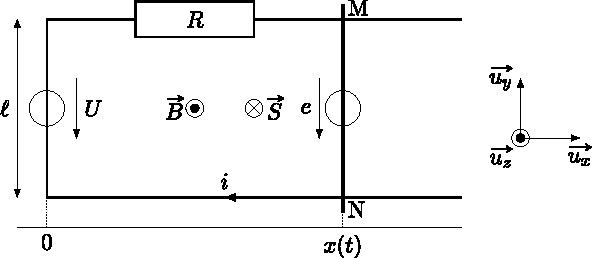
\includegraphics[scale=1, draft=true]{rlplgene_schema}
		}{
			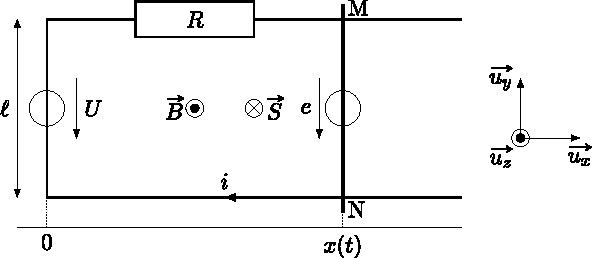
\includegraphics[scale=1]{rlplgene_schema}
		}%
		\captionof{figure}{Rails de \textsc{Laplace} générateurs.}
		\label{fig:rlplgene_schema}
	\end{center}
\end{minipage}

\subsubsection{Analyse qualitative}
\label{ssec:rlplgene_anaqual}
\begin{figure}[h]
	\centering
	\sswitch{
		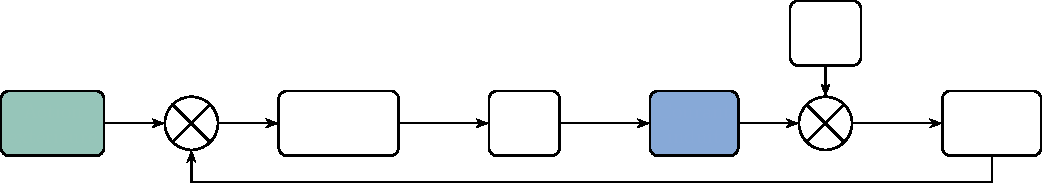
\includegraphics[scale=1]{modlenz-rlplgene_stud}
	}{
		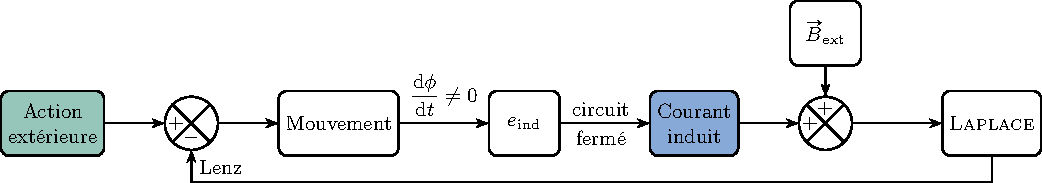
\includegraphics[scale=1]{modlenz-rlplgene_prof}
	}%
	\caption{Schéma de causalité des conséquences de l'induction.}
	\label{fig:modlenz_rlplgene}
\end{figure}
\begin{enumerate}
	\item À l'origine de l'induction est la présence d'un champ extérieur
	      $\vv{B\ind{ext}}$ et d'une action mécanique extérieure.

	\item Ce mouvement implique un \textbf{déformation} du circuit, et donc une
	      \textbf{variation du flux} et, d'après la loi de \textsc{Faraday}, une
	      f.é.m.\ induite y apparaît.

	\item Le circuit étant fermé, il y a donc également un courant induit, et avec
	      $\vv{B_{\ext}}$ il apparaît une action de \textsc{Laplace}.
\end{enumerate}

L'induction modérant, par ses conséquences, les causes qui lui ont donné
naissance, on en conclut que cette \textbf{action de \textsc{Laplace} s'oppose à
	la force initiale}, tendant à freiner le barreau.

\subsubsection{Analyse électrique}
\label{sssec:rlplgene_anaelec}
La déformation du circuit entraîne une variation de sa surface. Ainsi, même avec
un champ magnétique constant, le flux magnétique varie, impliquant l'apparition
d'une f.é.m.\ induite.
\bigbreak
\noindent
On fixe un sens pour $i$ (qui respecte cependant la loi de \textsc{Lenz}).
Avec $\vv{S} = -S\uz$ pris dans le sens de $i$, on trouve pour $\F$~:
\psw{%
	\[
		\F = B\uz \cdot -S\uz = -BS = -B \ell x
	\]
}%
D'où, avec la loi de \textsc{Faraday}~:
\psw{%
	\[
		e = -\dv{\F}{t} = B \ell \xp
	\]
}%
Placée en \textbf{convention générateur}. Donc, avec la loi des mailles~:
\psw{%
	\[
		e = Ri + U
		\qquad \Ra \qquad
		B \ell \xp = Ri + U
	\]
}%
Ainsi,
\begin{tcb*}(prop){Équation électrique}
	\psw{%
		\begin{equation}
			\usetagform{black}
			\label{eq:eqelecb}
			B \ell v = Ri + U
		\end{equation}
		\vspace*{-10pt}
	}%
\end{tcb*}

\begin{tcb}(rema)<lftt>'l'{Lien \textsc{Faraday}--\textsc{Lenz}}
	On peut observer le lien entre la loi de \textsc{Faraday} et la loi de
	\textsc{Lenz} par le signe «~$-$~»~: si $\xp > 0$, la surface augmente donc, en
	valeur absolue, le flux augmente.
	\smallbreak
	La loi de \textsc{Lenz} nous indique que le
	courant induit doit modérer cette augmentation, et donc créer un champ induit
	opposé au champ constant, donc dirigé selon $-\uz$~: on en déduit directement
	le sens réel de $i$.
	\smallbreak
	Avec la loi de \textsc{Faraday} et un choix arbitraire pour $i$, le signe
	moins nous donne directement que le flux diminue avec $x$, ce qui donne $e >
		0$ et effectivement $i > 0$~!
\end{tcb}

\subsubsection{Analyse mécanique}
\label{sssec:rlplgene_anameca}
On étudie le mouvement de la barre de masse $m$ dans le référentiel de la
salle de classe. Avec un bilan des forces~:
\begin{itemize}
	\item[b]{\psw{Poids}} \psw{%
		$\vv{P} = m \vv{g} = -mg\uz$~;
	}%
	\item[b]{\psw{Réaction normale}} \psw{%
		$\vv{N} = N\uz$~;
	}%
	\item[b]{\psw{Force opérante}} \psw{%
		$\vv{F} = F\ux$~;
	}%
	\item[b]{\psw{Frottements}} \psw{%
		$\vv{F_f} = -F_f \ux$ avec $F_f > 0$~;
	}%
	\item[b]{\psw{Force de \textsc{Laplace}}} \psw{%
		$\vv{F\ind{Lap}} = i \vv{\rm MN}\wedge \vv{B} = -i \ell B \ux$.
	}%
\end{itemize}
Ainsi,
\psw{%
	\[
		m \dv{\vv{v}}{t} = \vv{P} + \vv{N} + \vv{F} + \vv{F_f} + \vv{F\ind{Lap}}
	\]
}%
D'où, en projetant sur $\ux$~:
\begin{tcb*}(prop){Équation mécanique}
	\psw{%
		\begin{equation}
			\usetagform{black}
			\label{eq:eqmecab}
			m \dv{v}{t} = F - i \ell B - F_f
		\end{equation}
		\vspace*{-10pt}
	}%
\end{tcb*}

On a donc de nouveau deux équations couplées, reliant $v$ et $i$. On peut
obtenir une seule équation que l'on peut résoudre à partir des deux équations
obtenues, en utilisant l'équation électrique \eqref{eq:eqelecb} pour éliminer
$i$ de l'équation mécanique \eqref{eq:eqmecab}.

\subsubsection{Bilan énergétique}
\label{sssec:rlplgene_bilanrj}
\begin{itemize}
	\item[b]{Bilan mécanique}: \psw{%
		On multiplie le PFD par $v$~:
		\[
			mv \dv{v}{t} = Fv - i \ell Bv - F_fv
		\]
	}%
	On identifie~:
	\begin{itemize}
		\item puissance reçue par l'opérataire~: \psw{%
			      $\Pc\ind{ope}\sup{r} = Fv$
		      }%
		\item variation d'énergie cinétique de la barre~: \psw{%
			      $\dv{\Ec_c}{t} = mv \dv{v}{t}$
		      }%
		\item puissance fournie des forces de \textsc{Laplace}~: \psw{%
			      $\Pc\ind{Lap}\sup{f} = -\Pc\ind{Lap}\sup{r} = i \ell Bv$
		      }%
		\item puissance dissipée par frottements~: \psw{%
			      $\Pc_f\sup{f} = -(-F_fv) = F_f v$
		      }%
	\end{itemize}
	Ainsi,
	\psw{%
		\[
			\boxed{
				\Pc\ind{ope}\sup{r}
				=
				\dv{\Ec_c}{t} + \Pc_f\sup{f} + \Pc\ind{Lap}\sup{f}
			}
		\]
	}%
	\item[b]{Bilan électrique}: \psw{%
		On multiplie la LdM par $i$~:
		\[
			ei = Ui + Ri^2
		\]
	} On identifie~:
	\begin{itemize}
		\item puissance fournie par la f.é.m.~: \psw{%
			      $\Pc\ind{fem}\sup{f} = +ei = B \ell vi$
		      }%
		\item puissance dissipée par effet \textsc{Joule}~: \psw{%
			      $\Pc_J\sup{r} = Ri^2$
		      }%
		\item puissance reçue par le récepteur~: \psw{%
			      $\Pc_R\sup{r} = Ui = \Pc\ind{utile}$
		      }%
	\end{itemize}
	Ainsi,
	\psw{%
		\[
			\boxed{\Pc\ind{fem}\sup{f} = \Pc_J\sup{r} + \Pc_R\sup{r}}
		\]
	}%
\end{itemize}
\begin{tcb}(ror){Bilan de puissance électromécanique}
	On remarque ici aussi que
	\psw{%
		\[
			\boxed{\Pc\ind{fem}\sup{fournie} = \Pc\ind{Lap}\sup{fournie}}
		\]
	}%
	C'est-à-dire que le \textbf{couplage électromécanique est parfait}~: la
	puissance électrique fournie par la force électromotrice induite $(ei)$ est
	égale à la puissance mécanique fournie des forces de \textsc{Laplace}
	($-\Pc\ind{Lap}\sup{r} = i \ell Bv$).
\end{tcb}

\subsubsection{Bilan global}
\label{sssec:rlplgene_bilanglb}
En combinant les résultats de puissance, on a mathématiquement puis
schématiquement~:
\psw{%
	\[
		\boxed{
			\Pc\ind{ope}\sup{r} =
			\dv{\Ec_c}{t} + \Pc_f\sup{f} + \Pc_J\sup{r} +
			\underbracket[1pt]{\Pc\ind{utile}\sup{r}}_{Ui}
		}
	\]
}%
\begin{figure}[h!]
	\centering
	\sswitch{
		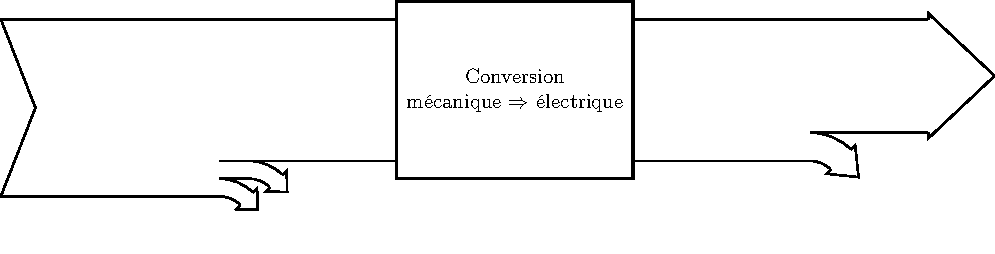
\includegraphics[width=\linewidth]{sankey_M-E_stud}
	}{
		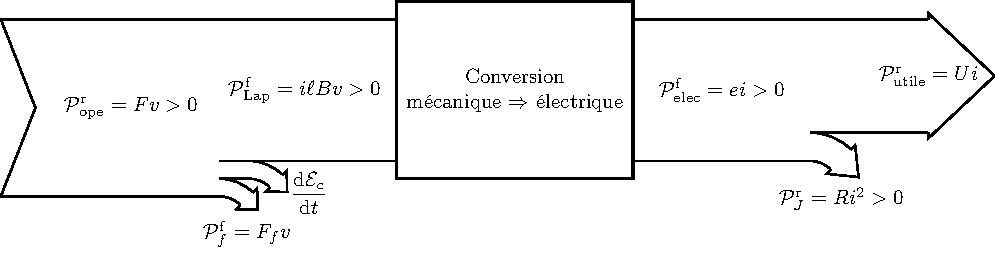
\includegraphics[width=\linewidth]{sankey_M-E_prof}
	}
	\vspace{-15pt}
	\captionof{figure}{Diagramme \textsc{Sankey} énergétique des rails de
		\textsc{Laplace} générateurs.}
	\label{fig:rlplgene_bilan}
\end{figure}

\newpage

Au travers de ces deux expériences, on en conclut donc que
\begin{tcb*}[list entry={\lte Conclusion conver$^\circ$ électromécanique}](ror)
	{Conclusion conversion électromécanique}
	\begin{itemize}
		\item \psw{%
			      La conversion de puissance électromécanique passe par des
			      \textbf{phénomènes d'induction}~;
		      }%
		\item \psw{%
			      La conversion est \textbf{réversible}~: même dispositif peut réaliser la
			      conversion dans un sens ou l'autre.
		      }%
		\item \psw{%
			      Le rendement de la conversion électromécanique n'\textbf{est pas borné par
				      un principe physique} et peut atteindre 1 en principe.
		      }%
	\end{itemize}
\end{tcb*}

\section{Exemples des convertisseurs}
\label{sec:exconv}
\subsection{Le moteur à entrefer plan}
\label{ssec:motentrefer}

La géométrie des rails de \textsc{Laplace} peut être modifiée pour obtenir un
moteur rotatif alimenté courant continu. Il se compose d'un \textbf{stator},
partie fixe constitué d'aimants qui produisent un champ magnétique stationnaire
$\vv{B_0}$, et d'un \textbf{rotor}, partie mobile constituée de $N$ files parant
dans la direction radiale et parcouru par un courant d'intensité $i$.
\smallbreak
\noindent
\hfill
\begin{minipage}[t]{.30\linewidth}
	~
	\begin{center}
		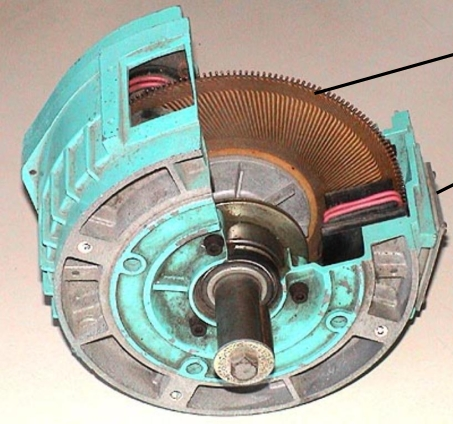
\includegraphics[scale=1.3]{mot_entrefer-phot}
		\captionof{figure}{Photo d'un moteur à entrefer plan.}
		\label{fig:motphoto}
	\end{center}
\end{minipage}
\hfill
\begin{minipage}[t]{.30\linewidth}
	~
	\begin{center}
		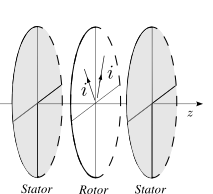
\includegraphics[scale=1]{mot_entrefer-olivier}
		\captionof{figure}{Schéma simplifié, vue de côté.}
		\label{fig:motolivier}
	\end{center}
\end{minipage}
\hfill~
\smallbreak

Ce dispositif peut s'utiliser de deux manières~:
\bigbreak
\noindent
\begin{minipage}[t]{.65\linewidth}
	\paragraph*{Fonctionnement moteur} On impose un courant $i$ dans chaque rayon,
	qui va du centre vers la périphérie. Chaque rayon sera comme un rail de
	\textsc{Laplace} moteur, créant des moments qui s'additionnent.
	\smallbreak
	\textit{Via} la loi de \textsc{Lenz}, ce mouvement va \textit{in fine} être à
	l'origine d'une f.é.m.\ induite, à l'origine d'un courant qui modèrera ce
	mouvement~: le rotor atteint une vitesse angulaire limite, proportionnelle à
	la tension d'alimentation.
\end{minipage}
\hfill
\begin{minipage}[t]{.30\linewidth}
	~
	\vspace{-40pt}
	\begin{center}
		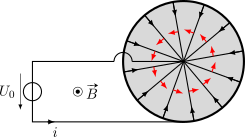
\includegraphics[width=\linewidth]{mot_entrefer}
		\captionof{figure}{Schéma électromécanique du moteur à entrefer.}
		\label{fig:motentre}
	\end{center}
\end{minipage}
\bigbreak
La vitesse de rotation de ces moteurs est très stable, le couple est indépendant
de la vitesse de rotation et du fait de la faible inertie du rotor, il
réagissent rapidement au changements de vitesse de rotation. Ils sont également
peu encombrants. En revanche, leur puissance est limitée à \SI{1}{kW}.

\noindent
\begin{minipage}[c]{.65\linewidth}
	\paragraph*{Fonctionnement générateur} On exerce sur la roue un couple
	$\Gamma_0$ afin de la forcer à tourner à une vitesse angulaire $\w$.
	\smallbreak
	Chaque rayon joue le rôle d'un rail de \textsc{Laplace} générateur, créant un
	courant induit à cause de la rotation dans le champ magnétique stationnaire
	$\vv{B_0}$.
\end{minipage}
\hfill
\begin{minipage}[c]{.30\linewidth}
	~
	\begin{center}
		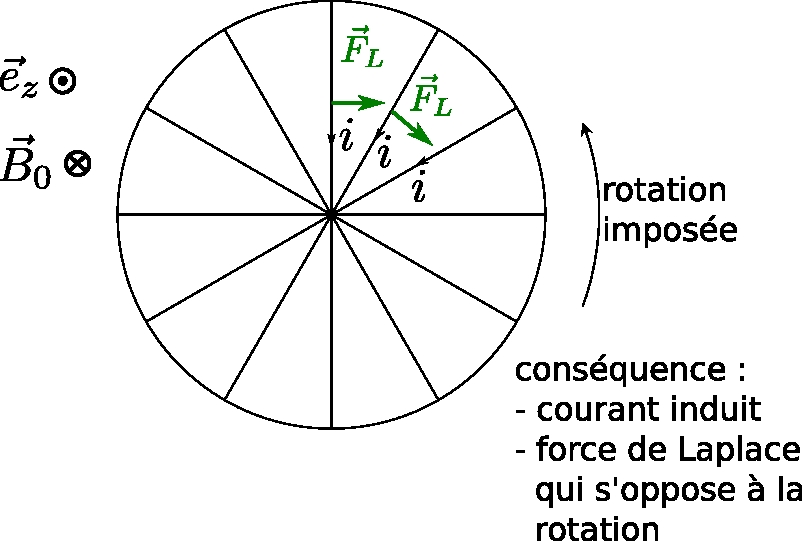
\includegraphics[width=\linewidth]{mot_entrefer-gene}
		\captionof{figure}{Schéma du moteur à entrefer en générateur.}
		\label{fig:motentrehene}
	\end{center}
\end{minipage}

\begin{tcb}(exem)<lftt>{au quotidien}
	\begin{itemize}
		\item motorisation des vélo et des chaises roulantes~;
		\item robotique industrielle~;
		\item médical (pompes à sang, dialyse).
	\end{itemize}
\end{tcb}

\subsection{Le haut-parleur électrodynamique}
\label{ssec:hpelectro}

\paragraph*{Cas particulier des ondes sonores} Le son étant une onde mécanique
(propagation de proche en proche de vibrations mécaniques dans un milieu), on
peut utiliser des phénomènes d'induction pour convertir un signal électrique en
un signal sonore (énergie mécanique).

\begin{tcb*}(defi){Haut-parleur et microphone}
	\begin{itemize}
		\item On parle de \textbf{haut-parleur} pour la conversion de puissance
		      \textbf{électrique} en puissance \textbf{sonore}.
		\item On parle de \textbf{microphone} pour la conversion de
		      puissance \textbf{sonore} en puissance \textbf{électrique}.
	\end{itemize}
\end{tcb*}

La géométrie des haut-parleurs rend difficile un calcul du flux magnétique à
travers un circuit déformable, néanmoins, on peut mettre en évidence
quelques-unes de ses caractéristiques sur un modèle très simple dans la
géométrie des rails de \textsc{Laplace}. Nous le ferons en TD.

\subsection{Freinage électromagnétique}
\label{ssec:electrofrein}
Dans le dispositif des rails de \textsc{Laplace}, la force de \textsc{Laplace}
s'oppose au mouvement de la barre, conformément à la loi de \textsc{Lenz}. En
l'absence d'opération externe pour maintenir le mouvement $(F=0)$~:
\[
	v\ind{lim} = 0
	\quad \Ra \quad
	\dv{v}{t} + \frac{v}{\tau} = 0
	\quad \Ra \quad
	v(t) = A\exp\left(-\frac{t}{\tau}\right)
\]
Cela conduit à une décroissance exponentielle de la vitesse de la barre sur un
temps $\tau$.
\smallbreak
\noindent
\begin{minipage}[c]{.60\linewidth}
	C'est le principe des ralentisseurs électromagnétiques utilisés sur les poids
	lourds. Dans un camion, il y a un disque solidaire de l'essieu qui tourne à la
	même vitesse angulaire que les roues.
	\smallbreak
	Sur demande de læ conductaire, un électroaimant peut générer un champ
	magnétique orthogonal au disque~: des courants induits apparaissent dans le
	volume du disque~: ces courants sont nommés \textbf{courant de
		\textsc{Foucault}}.
	\smallbreak
	Un couple proportionnel à $\w$ induit une décroissance exponentielle de la
	vitesse du camion.
\end{minipage}
\hfill
\begin{minipage}[c]{.35\linewidth}
	\begin{center}
		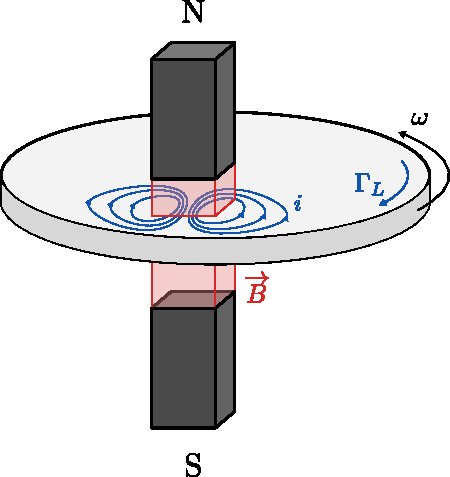
\includegraphics[width=\linewidth]{frein_induc}
	\end{center}
\end{minipage}

\paragraph*{Avantages}
\begin{itemize}
	\item \psw{%
		      pas de frottements solides, pas d'usure mécanique~;
	      }%
	\item \psw{%
		      les forces de \textsc{Laplace} sont réparties sur le volume, donc pas
		      d'échauffement localisé~;
	      }%
	\item \psw{%
		      pas de blocage de la roue~: vitesse nulle $\Ra $ pas de force de
		      freinage~;
	      }%
	\item \psw{%
		      possibilité de récupérer l'énergie créée.
	      }%
\end{itemize}
\paragraph*{Inconvénients}
\begin{itemize}
	\item \psw{%
		      freinage peu efficace à basse vitesse, ne permet pas au véhicule de
		      s'arrêter totalement puisque la décroissance est exponentielle (ou au bout
		      d'un temps très long).
	      }%
\end{itemize}

\section{Notions d'électrotechnique}
\label{sec:notelectrotech}
\subsection{Machine à courant continu}
\label{ssec:mcc}
On fabrique un moteur en plaçant un rotor constitué d'une spire rectangulaire
plongée dans le champ magnétique créé par deux aimants permanents (le champ
magnétique est supposé uniforme). La spire a une longueur $\ell $ et une largeur
$L$ et est parcourue par un courant $I$.
\begin{figure}[h]
	\centering
	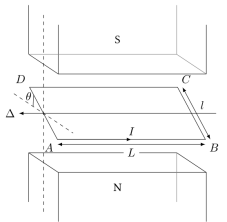
\includegraphics[scale=1]{mcc}
	\label{fig:mcc}
\end{figure}
Le champ magnétique est vertical, du Nord vers le Sud. On note $\uy$ son sens,
soit $\vv{B} = B\uy$, $\ux$ est la direction perpendiculaire à $\uy$ et l'axe
$\Delta{}$ de sorte que $(xy\Delta)$ soit directe.

\paragraph*{Couple des actions de \textsc{Laplace}}
La norme du moment magnétique est $m = iS$, donc sur $(\ux,\uy)$~:
\psw{%
	\[
		\vv{m} = iS \cos(\th)\uy + iS \sin(\th)\ux
	\]
	\vspace{-10pt}
}%
Soit le couple~:
\psw{%
	\[
		\Gf = \vv{m} \wedge \Bf = iSB\sin(\th) \ud
		\Ra
		\Gamma = iSB\sin(\th)
	\]
}%
\textit{A priori}, la spire se stabilise alors dans sa position d'équilibre $\th
	= 0$. Pour que ce système se comporte comme un moteur, on ajoute un mécanisme
qui permet d'\textbf{inverser le sens du courant à chaque demi-tour}. Ainsi, si
$0 < \th < \pi$, on a le même couple que précédemment, et si $\pi < \th < 2\pi$,
on a $\Gamma = -iS\sin(\th)$~; autrement dit,
\psw{%
	\[
		\boxed{\Gamma = iSB \abs{\sin(\th)}}
	\]
	\vspace{-10pt}
}%
Le couple moyen est alors
\psw{%
	\begin{align*}
		\moy{\Gamma}         & = iSB \moy{\abs{\sin(\th)}}_{[0,2\pi]}
		\\\Lra
		\Aboxed{\moy{\Gamma} & = \frac{4}{\pi} BSi}
	\end{align*}
	\vspace{-10pt}
}%
\begin{tcb*}(ror){Couple et intensité d'une MCC}
	On a alors un \textbf{couple proportionnel à l'intensité}~:
	\psw{%
		\[
			\moy{\Gamma} = KI
			\qav
			K = 4BS/\pi
		\]
	}%
\end{tcb*}

\paragraph*{Force électromotrice d'induction}
Le vecteur surface est
\psw{%
	\[
		\vv{S} = S\cos(\th)\uy + S\sin(\th)\ux
	\]
	\vspace{-10pt}
}%
Donc le flux
\psw{%
	\[
		\F = SB\cos(\th)
	\]
	\vspace{-10pt}
}%
Et la f.é.m.\
\psw{%
	\begin{align*}
		e         & = -\dv{\F}{t} = -BS \times \left( -\tp \sin(\th) \right)
		\\\Lra
		\Aboxed{e & = BS\w \sin(\th)}
	\end{align*}
}%
Lorsque $\pi < \th < 2\pi$, la tension est inversée par le collecteur, de sorte
que la tension aux bornes de la machine soit $u = -e = -BS\w\sin(\th)$. Et donc,
quel que soit $\th$~:
\psw{%
	\[
		\boxed{u = BS\w \abs{\sin(\th)}}
	\]
}%
Et la tension moyenne~:
\psw{%
	\begin{align*}
		\moy{u}         & = BS \w\moy{\abs{\sin(\th)}}_{[0,2\pi]}
		\\\Lra
		\Aboxed{\moy{u} & = \frac{4}{\pi} BS\w}
	\end{align*}
}%
\begin{tcb*}[list entry={\lte Tension et vitesse ang.\ d'une MCC}](ror)
	{Tension et vitesse angulaire d'une MCC}
	On a alors une \textbf{tension proportionnelle à la vitesse angulaire}~:
	\psw{%
		\[
			\moy{u} = K\w
			\qav
			K = 4BS/\pi
		\]
	}%
\end{tcb*}
\begin{tcb*}(impl){Fonctionnement d'une MCC}
	Par une rapide étude en puissance, on trouve
	\[
		\psw{%
			uI = K\w I = K\w \frac{\Gamma}{K} = \Gamma\w
			\quad
			\Lra
			\Pc\ind{elec} = P\ind{Lap}
		}%
	\]
	On peut donc facilement \textbf{adapter la charge} en jouant sur l'intensité.
\end{tcb*}

\begin{tcb*}(rema)<lftt>'l'{Inconvénient principal}
	Ce moteur présente l'inconvénient d'imposer une couple variable en
	fonction de $\th$ (le couple est nul pour certaines positions et ne peut
	démarrer dans ces positions). Les moteurs réels ont donc un champ
	magnétique radial pour avoir un couple constant.
\end{tcb*}

\subsection{Champ magnétique tournant}
\label{ssec:chptournant}
\begin{figure}[H]
	\centering
	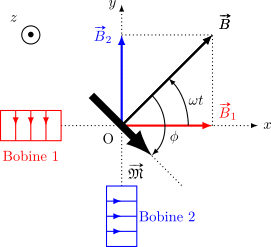
\includegraphics[scale=1]{chptournant}
	\label{fig:chptournant}
\end{figure}

On place deux bobines à $\ang{90}$ l'une de l'autre. La bobine 1 est parcourue
par un courant $i_1 = i_0\cos(\wt)$, et la bobine 2 par un courant $i_2 =
	i_0\sin(\wt)$.
Le champ produit par la bobine 1 est $\vv{B_1} = B_0\cos(\wt)\ux$, et par la
bobine 2 est $\vv{B_2} = B_0\sin(\wt)\uy$, en déphasage de $\pi/2$. Le champ
total au centre est donc
\psw{%
	\[
		\vv{B} = B_0(\cos(\wt)\ux + \sin(\wt) \uy)
	\]
}%
c'est-à-dire un champ magnétique tournant. En plaçant un aimant au centre de ce
champ, comme il a tendance à s'aligner sur le champ, il va se mettre à tourner~:
on a construit un moteur, dit \textbf{moteur synchrone}.
\bigbreak
En pratique, on utilise des tensions triphasées, c'est-à-dire trois signaux de
tensions~:
\begin{gather*}
	U_0(t) = U\cos(\wt)
	\\
	U_1(t) = U\cos( \wt + \frac{2\pi}{3} )
	\\
	U_2(t) = U\cos( \wt + \frac{4\pi}{3} )
\end{gather*}
avec trois bobines placées à des angles $0, 2\pi/3$ et $4\pi/3$.

\end{document}
